\chapter{Introduction}
This thesis is based on part of the EPI-project, developed at Barcelona Supercomputing Center, in particular on the V-Extension implementation.
In this Chapter there will be presented and discussed all the RISC-V and V-Extension concepts, but they will be not covered all the topics regarding the RISC-V ISA or all the extensions, as they are not always relevant to the project.\\
Starting from the Concepts there will be also an explaination on the context of the project, so the real implementation and application of the ISA specifications.
In particular there will be a exposition of Verification concepts and on the UVM structure, filled by the details useful to understand the work done.



\section{Concepts}
\subsection{RISC-V}
RISC-V is an open, extensible and free instruction set architecture (ISA). It was originally designed to support computer architecture research and education\cite{RISC-V-Instruction-Set-Manual}.\\
The project began at the Berkley, University of California in 2010, and then in 2011 was published the first ISA User Manual. After that there was the first tapeout of a RISC-V chip in 28nm FDSOI donated by STMicroelectronics.\\

The RISC-V ISA is implemented as a base integer ISA, but it is modular and so supports  variable-length instruction encodings.\\
This ISA is provided under open source licenses, and it is gaining a lot of popularity due to its open nature. \\
Mainly there are two primary base integer variants, RV32I and RV64I, which provide 32-bit or 64-bit user-level address spaces respectively.\\

RISC-V is designed to have good customization and so it's provided with the possibility to be extended, but the base integer instructions cannot be redefined.\\
There are two kinds of extensions:
\textit{standard} and \textit{non-standard}.
\begin{itemize}
    \item The \textit{standard} ones need to be compatible with all the other standards and also they should aim to be generally useful.
    \item The \textit{non-standard} ones can be highly specialized in some task and so can be in conflict with other extensions.
\end{itemize}

For general development some standard extensions are predefined:
\begin{itemize}
    \item "\textbf{I}" is the base integer extension and contains integer computational instructions, integer loads, integer stores, and control-flow instructions. It is mandatory for all RISC-V implementations.
    
    \item "\textbf{M}" is the standard integer multiplication and division extension, it allows to multiply and divide the values held in the integer registers.
    
    \item "\textbf{A}" is the standard atomic instruction extension. For inter-processor synchronization is useful to have atomic instructions so with this extension is possible to read, modify, and write memory atomically . 
    
    \item "\textbf{F}" is the standard single-precision floating-point extension. It adds floating-point registers, single-precision computational instructions, and single-precision loads and stores. 
    
    \item "\textbf{D}" The standard double-precision floating-point extension. It is useful when the F extension is not enough, so expands it and adds double-precision computational instructions, loads, and stores.
    
    \item "\textbf{G}" is the denotation for an integer base plus these four standard extensions (“IMAFD”).
\end{itemize}


The design philosophy of the RISC-V projects is based on modularity: the base ISA will not change over time, but new extensions will be available and new feature will be added. This is useful because is very difficult to find general useful extension beyond the ones already exist. So it wouldn't be convenient to constantly add new features to the base ISA and then have to keep track of that.\\
In Figure \ref{riscv-base-instruction-formats} it is possible to see how the base instruction are composed.

\begin{figure}[h]
    \centering
    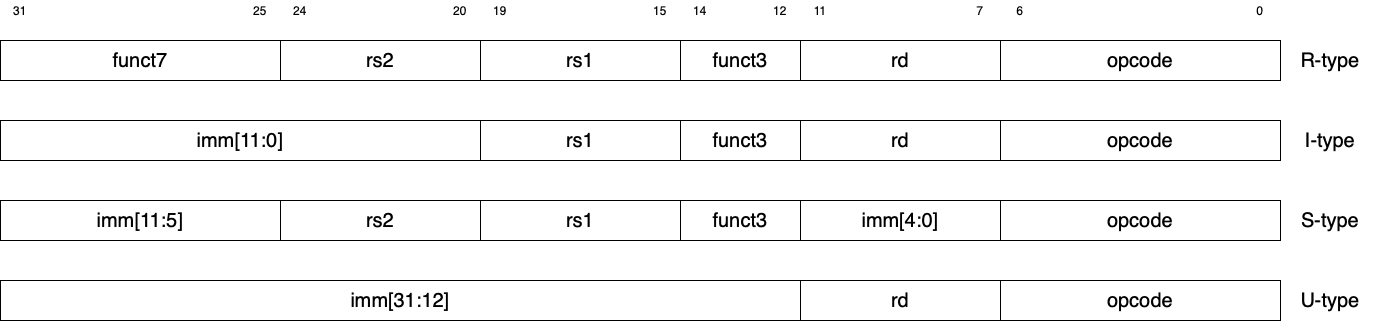
\includegraphics[scale = 0.27]{Chapter_1/img/riscv-base-instruction-formats.png}
    \caption{RISC-V base instruction formats. Each immediate subfield is labeled with the bit position (imm[x]) in the immediate value being produced, rather than the bit position within the instruction’s immediate field as is usually done.\cite{RISC-V-Instruction-Set-Manual}}
    \label{riscv-base-instruction-formats}
\end{figure}

It is important to notice that RISC-V is a load-store architecture, this means only load and store operations can have access to the memory.\\
It is a very convenient organization, because it reduces the average time-per-operation and guarantees a good functioning of the pipelined structure.\\

It also supports signed byte and half word loads, which is very useful when  working with signed byte and half word data types.

In Figure \ref{riscv-load-store} it is possible to see how the load-store instructions are composed.

\begin{figure}[h]
    \centering
    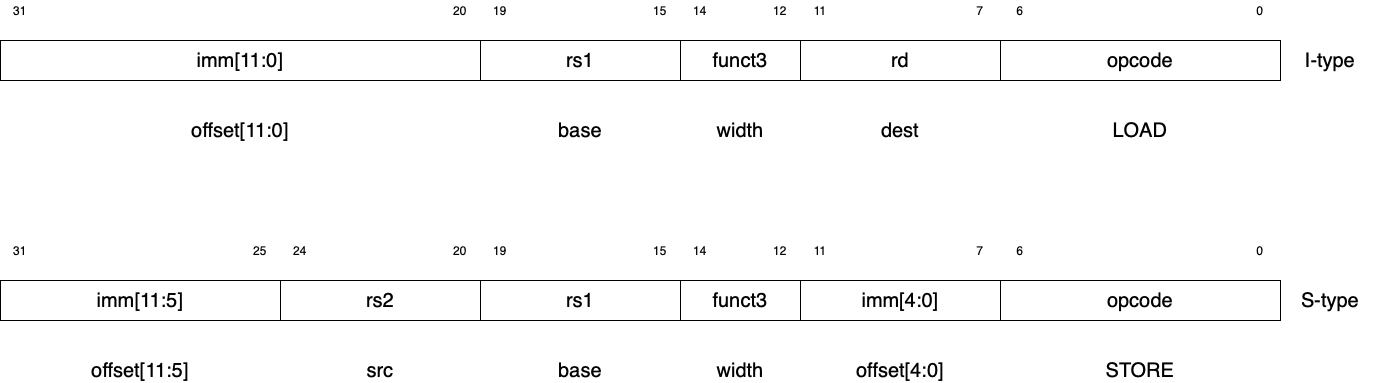
\includegraphics[scale = 0.27]{Chapter_1/img/riscv-load-store.png}
    \caption{RISC-V load/store instruction formats. It is possible to see that the LOAD is a I-type op and the STORE is an S-type op. \cite{RISC-V-Instruction-Set-Manual}}
    \label{riscv-load-store}
\end{figure}


\subsection{Vectors and RISC-V V-Extension}

%% chapter 10 and 15

%%https://www.european-processor-initiative.eu/v-for-vector-software-exploration-of-the-vector-extension-of-risc-v/

%%github risc-v 0.7.1
\subsection{Verification}
%% Ray Ray


\section{Context}
\subsection{The VPU}
\subsection{The UVM}
\subsection{Submodules and checkers}